%\addcontentsline{toc}{chapter}{Appendix}
%\begin{appendices}
%\appendix
%\counterwithin{figure}{section}
%\counterwithin{table}{section}
\section{Data Summary} \label[appendix]{sec:overall_analysis}
\begin{figure}[ht!]
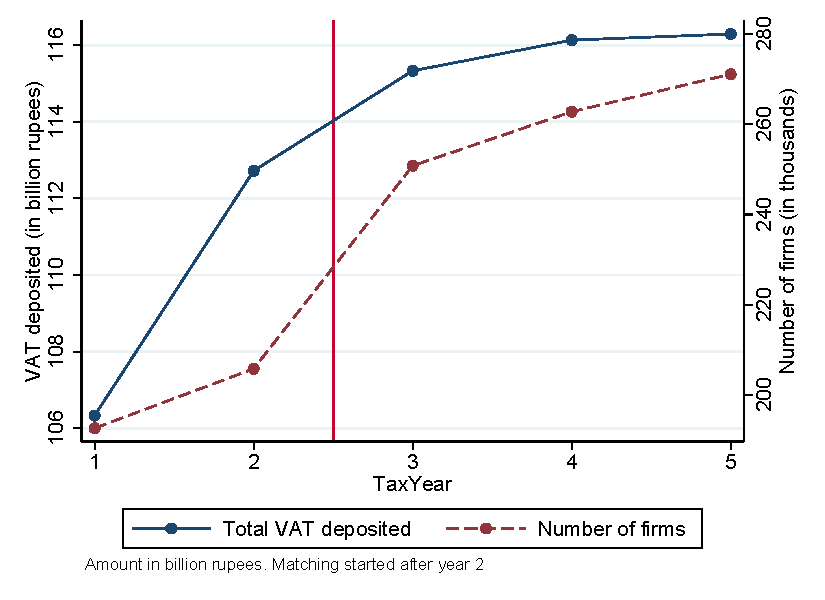
\includegraphics[width=.6\textwidth]{graphs/TotalVATDeposited_ALL_Real.pdf}
\caption{Total VAT Remitted (For All Firms)}  
\label{fig:vatdeposited-all}
\floatfoot{\scriptsize The third party verification policy began at the beginning of year 3. VAT remitted increases from \rupee 106.33 billion in year 1 to \rupee 116.29 billion in year 5. This is an average annual growth rate of 1.8\% in real terms as compared to a real state level GDP growth rate of about 5.7\% (Source:\citep{delhihandbook2015}). The y axis is in billion rupees, where 1\$ roughly equals \rupee 65.Values have been adjusted to year 1 price terms.}
\end{figure}

In this section, we describe the distribution of the firms registered in the Delhi VAT system. In \cref{fig:vatdeposited-all}, we plot the total VAT collections and the total number of firms registered for VAT across the 5 years. The third-party verification policy was implemented at the beginning of year 3. VAT deposits increase from \rupee 106.33 billion in year 1 to \rupee 116.29 billion in year 5. This is an average annual growth rate of 1.8\% in real terms as compared to a real state level GDP growth rate of about 5.7\%. We note that the number of registered firms go up sharply after the policy change which implies that average collections per firm actually decrease. We believe that this increase in the number of firms is driven by unrelated policy changes. Specifically, before quarter 2 of year three, firms had to deposit a surety amount between \rupee 50,000 to \rupee 100,000 as part of registration. The tax authority relaxed this restriction with the goal of improving ``ease of doing business'' from the second quarter of year three onwards.


\begin{figure}[t!] 
%\centering
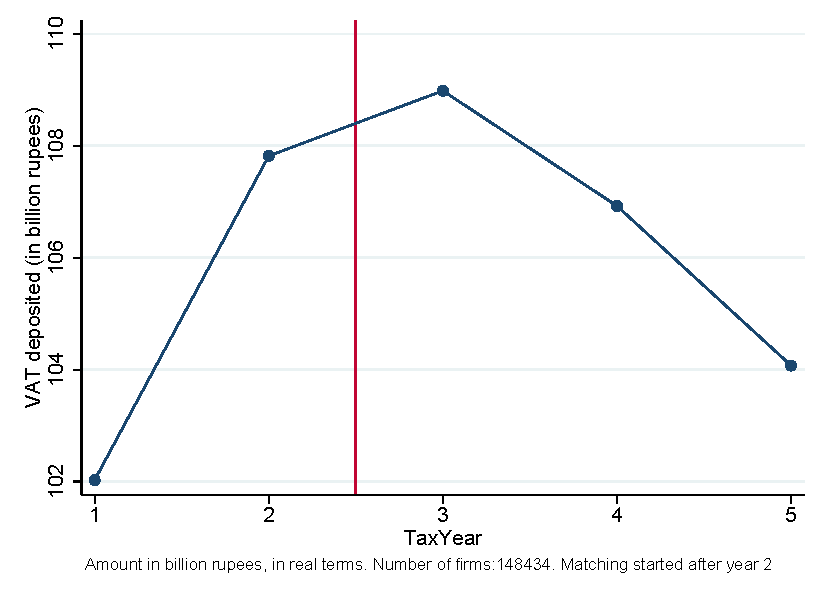
\includegraphics[width=.6\textwidth]{graphs/TotalVATDeposited_TotalCount5_Real.pdf}
\caption{Total VAT Remitted (For Firms That are Present in All Years)}
\floatfoot{\scriptsize Total collection trends for firms that are present in all the years of our sample period. There are 148434 such firms. The y axis is in billion rupees, where 1\$ roughly equals \rupee 65. Values have been adjusted to year 1 price terms. VAT remitted increases from \rupee 102.02 billion in year 1 to \rupee 104.07 billion in year 5.}
\label{fig:vatdeposited-alwayspresent}
\end{figure}

The number of firms filing a return increases from 192,664 in year 1 to 271,090 in year 5. There is a wide variation in the amount deposited. To begin with, only about 50\% of registered firms remit a positive VAT in any given filing period. Further, between 7 and 15\% of the firms (depending upon the tax period) that file a return report a zero turnover (sales). Furthermore, between 5 and 9\% of the firms declare their entire turnover to consist of interstate (or non-local) sales and about 32\% firms declare their entire turnover to be purely local (refer to \Cref{tbl:all-summary}). Note that the third party verification mechanism breaks down for inter-state sales since the transacting firm's returns are submitted to a different tax authority and to date there has been little coordination between different tax jurisdictions on such cross-checking.\footnote{The GST bill legislated by the central and state governments will unify the tax administration and make it much easier to cross-check inter-state transactions.} 

\begin{figure}[t!]
%\scriptsize
%\centering
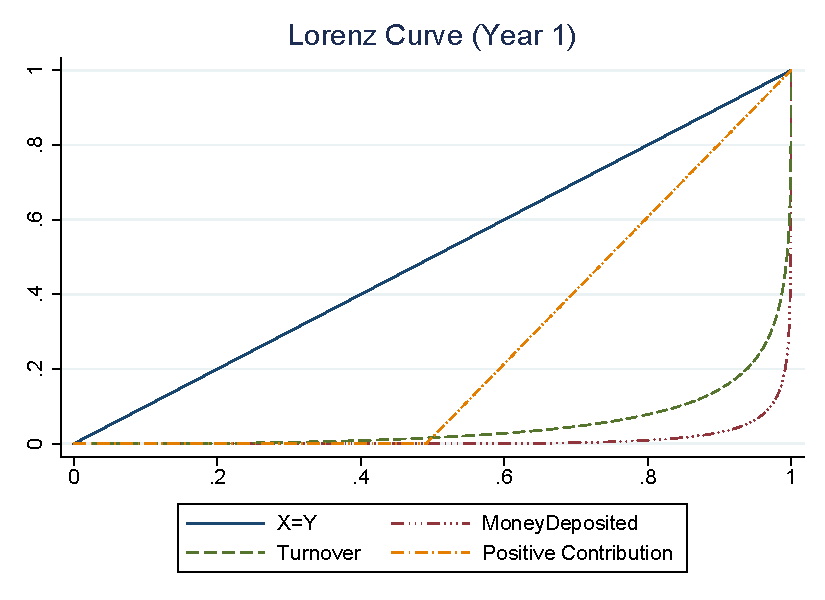
\includegraphics[width=.6\textwidth]{graphs/LorenzCurve_TaxYear1.pdf}
\caption{Lorenz Curve for All Firms in Tax Year 1}
\label{fig:lorenzyear1}
\floatfoot{Note: Only 50\% of firms deposit any taxes, and 5\% of firms provide 95\% of total collections. Lorenz curve for all the firms in year 1 of our dataset (returns collated at annual level).}
\end{figure}


\begin{table}[t!]
\footnotesize
%\scriptsize
\scalebox{0.85}{
\begin{threeparttable}
\begin{tabular}{lcccccc}\\ 
\hline \hline
(1)&(2)&(3)&(4)&(5)&(6)&(7)\\
Year & No. of Firms & VAT Remitted & \% Positive VAT  & \% Zero-Turnover  & \% Interstate & \% Local Firms \\  
& & & Deposited Firms & Firms &Firms & \\ \hline
1&192664& 106330.3 &50.88&7.10&9.03&31.26 \\
2&205832&112720.1&48.72&9.51&7.72&31.40 \\
3&250805&115330.6&47.57&15.05&5.94&31.68 \\
4&262775&116132.1&49.70&13.68&5.70&32.70 \\
5&271090&116292.4 &53.60&13.98&6.00&32.64 \\ \hline \hline
\end{tabular} 
\begin{tablenotes}[para,flushleft]
\scriptsize
Summary of all the firms that filed a return in the given year. Column (3) shows total VAT collected by the tax authority from all firms in that year in million rupees, with \rupee 65 approximately equal to \$1. Column (4) shows percentage of firms that deposited a positive amount of VAT. Column (5) show percentage of firms which filed a return but declared a turnover of zero. Column (6) shows percentage of firms that had a non-zero turnover and entire sales were interstate. Column (7) shows percentage of firms who had a non-zero turnover and all sales were local. For example, in year 1, 31.26\% firms had only local sales, 9.03\% had only interstate sales, and 7.1\% had a turnover of 0. Therefore, roughly 53\% of the firms had a non-zero turnover and had declared both local as well as inter-state sales.
\end{tablenotes}
\caption{Summary Stats: All Firms}
\label{tbl:all-summary}
\end{threeparttable}}
\end{table}

In \cref{fig:lorenzyear1,fig:lorenzyear5} we plot Lorenz curves for (a) total turnover, (b) VAT remitted, and (c) a dummy for any positive VAT remitted separately for year 1 and 5 of the study. Inequality in contributions is stark with the top 5\% of firms remitting roughly 95\% of the total VAT collected by the tax authority. The number of firms that remit any VAT is surprisingly low, with the number hovering around 50\% across the 5 years.

\begin{figure}[t!]
\scriptsize
\centering
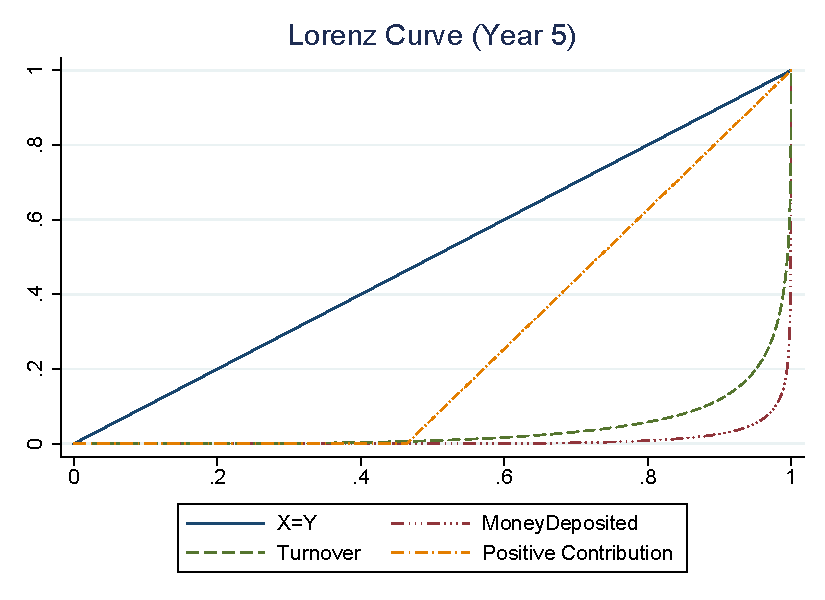
\includegraphics[width=.6\textwidth]{graphs/LorenzCurve_TaxYear5.pdf}
\caption{Lorenz Curve for All Firms in Tax Year 5}
\label{fig:lorenzyear5}
\end{figure}

In \cref{fig:vatdeposited-alwayspresent} we focus our attention on firms which are present in all 5 years of our dataset i.e. we drop firms that enter or exit during our time-frame of interest. There are 148,434 such firms which remit roughly 95\% of our total tax collections in year 1 and 89\% of the tax collections in year 5. VAT remits from these firms go from \rupee 102.02 billion in year 1 to \rupee 104.07 billion in year 5 (for a real growth rate of 0.39\%). In this set of firms, the percentage of firms remitting a positive amount goes up marginally, compared to all firms, to about 57\%. The percentage of firms that declare a turnover of zero is between 2.5 to 8.5\% across the 5 years. The percentage of firms doing only interstate sales and only local sales is also comparable to the entire sample (refer to \cref{tbl:always_summary}). To conclude, our estimation sample comprises the bulk of the tax collections for the state throughout the study period. 

\begin{table}[t!]
\footnotesize
%\scriptsize
\begin{threeparttable}
\begin{tabular}{cccccc}\\ \hline \hline
(1)&(2)&(3)&(4)&(5)&(6)\\
Year & VATDeposited & \% Positive VAT  & \% Zero-Turnover & \% Interstate & \% Local Firms \\  
& & Deposited Firms & Firms &Firms & \\ \hline
1& 102024.5 &54.60&2.50&6.97&30.76 \\
2&107820.3 &54.09&3.09&5.95&31.14 \\
3&108985.1 &57.20&3.88&5.34&30.61 \\
4&106926.4&57.50&5.35&5.18&30.45 \\
5&104071.8 &60.49&8.50&5.22&29.74 \\ \hline \hline
\end{tabular} 
\begin{tablenotes}[para,flushleft]
  Summary of firms that filed a return in all the 5 years for which we have the data (2010-11 to 2014-15). Number of such firms in our sample is 148434. Column (2) shows total VAT remitted by the tax authority from all firms in that year in million rupees, with \rupee 65 approximately equal to \$1. Column (3) shows percentage of firms that remitted a positive amount of VAT. Column (4) show percentage of firms which filed a return but declared a turnover of zero. Column (5) shows percentage of firms that had a non-zero turnover and entire sales were interstate. Column (6) shows percentage of firms who had a non-zero turnover and all sales were local. For example, in year 1, 30.76\% of the 148434 firms that are present in all the years of our sample, had only local sales, 6.97\% had only interstate sales, and 2.5\% had a turnover of 0. Therefore, roughly 60\% of the firms had a non-zero turnover and had declared both local as well as inter-state sales.
\end{tablenotes}
\caption{Summary stats: Always Present Firms}
\label{tbl:always_summary}
\end{threeparttable}
\end{table}


\pagebreak


\section{Quarterly Results}
\label[appendix]{sec:quarterlyresults}

\subsection{Quarterly Analysis Along with Falsification Test}
\label[appendix]{subsec:falsification-test}

\begin{figure}[ht!] 
\caption{Wholesalers vs Retailers: Quarterly Trends}
\label{fig:group1-pretrends-quarterly}
\centering
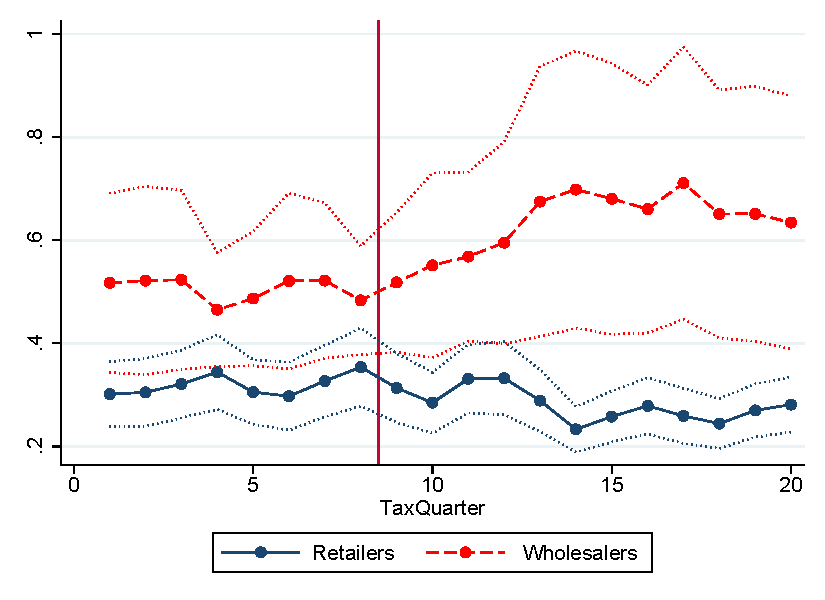
\includegraphics[width=.75\textwidth]{graphs/MeanMoneyDeposited_quarterly_with_confidenceintervals_Real.pdf}
\floatfoot{\footnotesize $N_W=11482$, $N_R=15337$. VAT remitted is in million rupees, with \rupee 65 approximately equal to \$1. VAT remitted has been inflation adjusted to Q1-2010-11 price levels. Sample smaller than the annual frequency sample because in year 1 and year 2 firms with turnover less than 5 million had to file at annual or semi-annual frequency.}
\end{figure}

In addition to the basic model explained in \cref{subsec:identification_model}, we carry out robustness check by the falsification test described below. In \cref{eq:basic}, we now add a $Pre_{it}$ dummy which is equal to 1 if the quarter is 7 or 8 i.e. just before the introduction of the third party verification policy. We also interact the $Pre_{it}$ dummy with $\mathbb{I}\{\text{Wholesaler}_{i}\}$ which is a dummy for the firm i being a wholesaler. The falsification test is provided by coefficient $\mu$ corresponding to the interaction between $Pre_{it}$ dummy and $\mathbb{I}\{\text{Wholesaler}_{i}\}$ dummy. The coefficient indicates whether, before the introduction of the policy, the outcome variable is evolving similarly between wholesalers and retailers during the 2 quarters before the introduction of the policy. Consistent with the quarterly event-study analysis (\cref{fig:eventstudy-figure-quarter}), the pre-policy effect on wholesalers is close to zero, precisely estimated,\footnote{The standard errors are smaller than those for $\gamma$ coefficient.} and statistically insignificant. Results shown in \cref{tbl:event-falsification-table}.

\begin{multline} \label{eq:falsification}
 y_{it}=\alpha_i+\nu_t+\beta*Post_{it}+\delta*Pre_{it}+\gamma*Post_{it}*\mathbb{I}\{\text{Wholesaler}_{i}\} \\
  +\mu*Pre_{it}*\mathbb{I}\{\text{Wholesaler}_{i}\}+\epsilon_{it}
\end{multline}

\begin{table}[t!]
\scalebox{0.75}{
\begin{threeparttable}
\centering 
\footnotesize
\caption{Falsification Test: Wholesalers and Retailers (Quarterly)}
\label{tbl:event-falsification-table}
 \begin{tabular}{lccccc} \hline \hline
     & (1) & (2) & (3) & (4) & (5)  \\
VARIABLES & Positive VAT  & VAT Remitted & Tax Credit & Output Tax & Output Tax -\\
   & Remitted &  &  & & Tax Credit\\ \hline
Post*Wholesaler & -0.0147*** & 0.158*** & -0.0240 & 0.132*** & 0.156*** \\
 & (0.00355) & (0.0491) & (0.0496) & (0.0392) & (0.0501) \\
PrePolicy*Wholesaler & -0.00278 & -0.0312 & 0.0385 & 0.00530 & -0.0332 \\
 & (0.00372) & (0.0304) & (0.0308) & (0.0269) & (0.0320) \\
\hline
Post & 0.0139***  & -0.0604* & 0.0382* & -0.0194 & -0.0576** \\
 & (0.00349)  & (0.0322) & (0.0220) & (0.0392) & (0.0289) \\
PrePolicy & 0.0189***  & 0.0288 & 0.0637*** & 0.0928*** & 0.0291 \\
 & (0.00352) & (0.0210) & (0.0240) & (0.0359) & (0.0201) \\
\hline
Mean Dep.Var. & 0.44 & 0.52 & 0.54 & 1.02 & .48 \\
&(0.00)& (0.09)&(0.15)&(0.22)&(0.09) \\ \hline
Observations & 536,380 & 536,380 & 536,380 & 536,380 & 536,380 \\
R-squared & 0.549 & 0.86 & 0.78 & 0.96 & 0.86 \\ 
Number of Firms & 26,819 & 26,819 & 26,819 & 26,819 & 26,819 \\ \hline \hline
\end{tabular}
  \begin{tablenotes}[para,flushleft]
\footnotesize Robust standard errors in parentheses, clustered at firm level. $N_W=11482$, $N_R=15337$. Monetary amounts are in million rupees, inflation adjusted to price levels of Q1 of 2010-11, with \rupee 65 approximately equal to \$1. Column (1) shows linear probability regression of the probability of remitting a positive amount. Column (2)-(4) respectively show regression of the mean VAT remitted by firms, of the input tax credit claimed by firms, and the output tax collected by firms. To address the concern that VAT remitted has a significant mass at zero, column(5) shows regression of the difference between output tax and input credit declared by firms. Dependent variables have been price adjusted in Q1 of 2010-11 terms. Row ``Mean Dep.Var.'' shows mean and standard errors for wholesalers in quarter 1. *** p$<$0.01, ** p$<$0.05, * p$<$0.1
\end{tablenotes}
\end{threeparttable}}
\end{table}


\pagebreak

\section{Flexible DID Specifications}
\label[appendix]{sec:eventstudy-analysis}

\subsection{Econometric Model of Event Study Analysis}
\label[appendix]{subsec:eventstudy-econometrics}
We can take advantage of the large N and moderate T dimensions in our data set to estimate richer treatment effect models. In particular, we can examine flexibly the differential evolution of outcomes between wholesalers and retailers over the entire time-period under study. In particular, we estimate \cref{eq:flex} as outlined in
\cref{subsec:identification_model}. We normalize $\gamma_2$ in that equation ($\gamma_8$ for quarterly analysis) to zero so that the coefficients $\{\gamma_s\}_{s \in S }$ measure differential changes in the outcome and relative to the year (quarter) prior to the policy introduction.

We report the coefficients in graphical form, with their corresponding 95\% confidence intervals (see for example \cref{fig:eventstudy-figure-annual}). If the coefficients $\{\gamma_s\}_{s>2}$ (i.e., the coefficients after the introduction of the third party verification) are positive, that implies that outcomes increase on average for wholesalers relative to retailers after the policy introduction. If $\gamma_s$ is positive only for some $2 < s \leq \bar{s} \leq 5$, then the increase in outcomes is transitory, lasting up to $\bar{s}$ years after the policy introduction. If the coefficient $\gamma_1$ (i.e., the coefficient in the figure to the left of the policy introduction) is positive, then the outcome variable was declining  before the introduction of the policy. 

To formally test the hypothesis that pre-policy trends between wholesalers and retailers are not different, we test the null hypothesis $\gamma_1=\gamma_2=..=\gamma_{l-1}=0$ where l denotes the time period in which the automatic third party verification policy was introduced. For the analyses below (carried out for the quarterly and annual frequencies) we cannot reject that pre-treatment trends are equal between wholesalers and retailers.  

%\pagebreak

\begin{table}[t!]
\footnotesize
\begin{threeparttable}
\begin{tabular}{lllll} \hline \hline
 & (1) & (2) & (3) & (4) \\
VARIABLES & Annual & Quarter & Top Decile &Top Decile  \\ 
 &  &  & (Annual) & (Quarter)  \\ \hline
Positive VAT Deposited & 0.68  & 0.27 & 0.02 &0.00 \\
VAT Deposited & 0.61 &  0.20 & 0.46 &0.27 \\
Tax Credit & 0.12 & 0.36 & 0.69 & 0.43 \\
Output Tax & 0.23 & 0.65 & 0.98 & 0.28 \\
Output Tax - Tax Credit & 0.56 & 0.54 & 0.56 & 0.69 \\ \hline
\end{tabular}
\begin{tablenotes}[para,flushleft]
To formally test the hypothesis that pre-policy trends between wholesalers and retailers are not different, we test the null hypothesis $\gamma_1=\gamma_2=..=\gamma_{l-1}=0$ where l denotes the time period in which the automatic third party verification policy was introduced. l is 3 in column (1) and (3), and 9 in column (2) and (4). Column (1) does the test for returns data at annual frequency, column (2) does the test for returns at quarterly frequency, and column (3) and (4) do the test for returns data at annual and quarterly frequency but only for firms in the top decile (of both retailers and wholesalers) of VAT remitted in year/quarter 1.
\end{tablenotes}
\caption{Pre-trend Analysis: Wholesalers vs Retailers}
\label{tbl:}
\end{threeparttable}
\end{table}

%\pagebreak

\subsection{Annual Analysis}
\label[appendix]{subsec:eventstudy-annual}
\begin{figure}[H]
\centering
\subfloat[VAT Deposited]{
  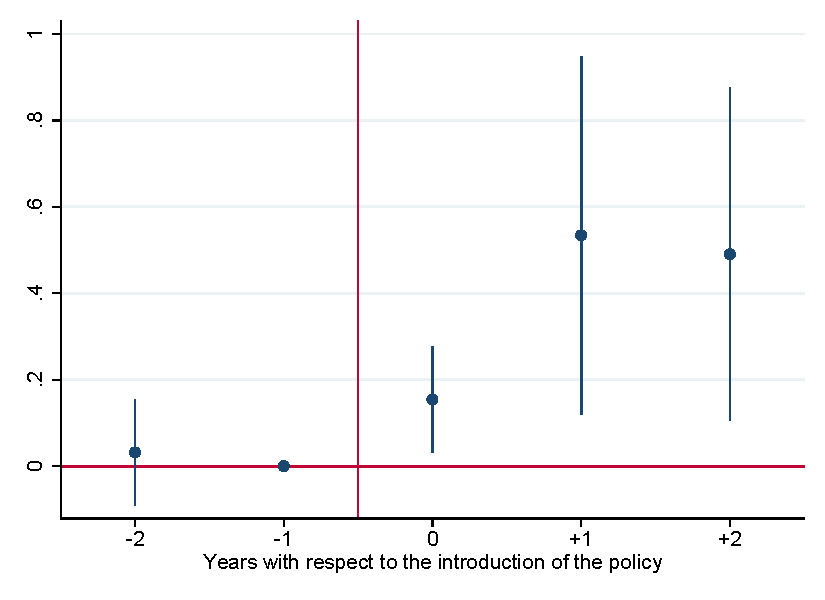
\includegraphics[width=47.2mm]{graphs/EventStudy-MoneyDeposited-Annual-Real.pdf}
  \label{fig:eventstudy-figure-annual-vatdeposited}
}
\subfloat[Output Tax - Input Credit]{
  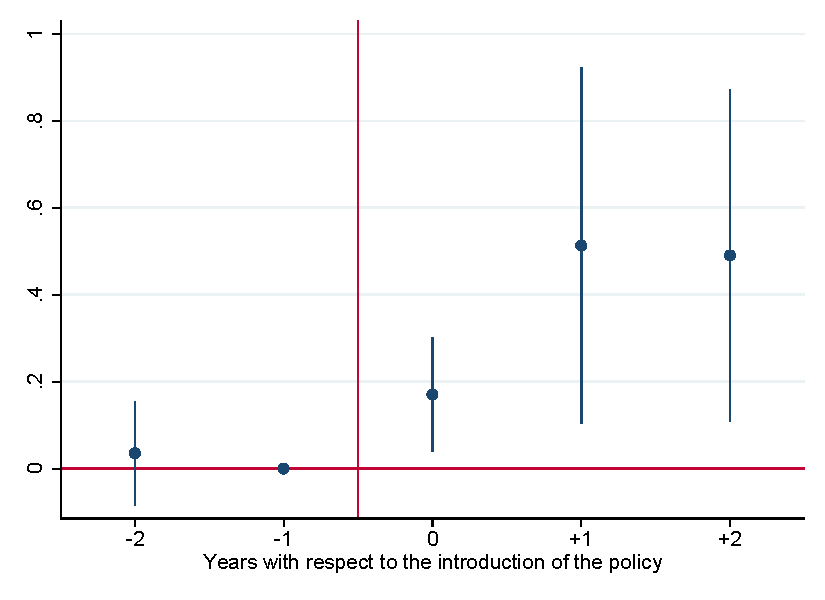
\includegraphics[width=47.2mm]{graphs/EventStudy-Diff-Annual-Real.pdf}
   \label{fig:eventstudy-figure-annual-diff}
}
\hspace{0mm}
\subfloat[Output Tax]{
  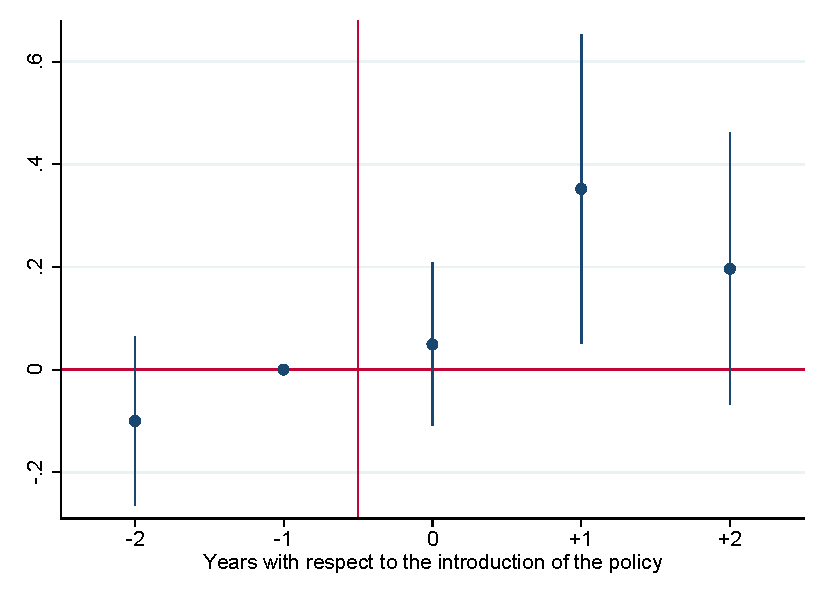
\includegraphics[width=47.2mm]{graphs/EventStudy-OutputTax-Annual-Real.pdf}
   \label{fig:eventstudy-figure-annual-outputtax}
}
\subfloat[Input Credit]{
  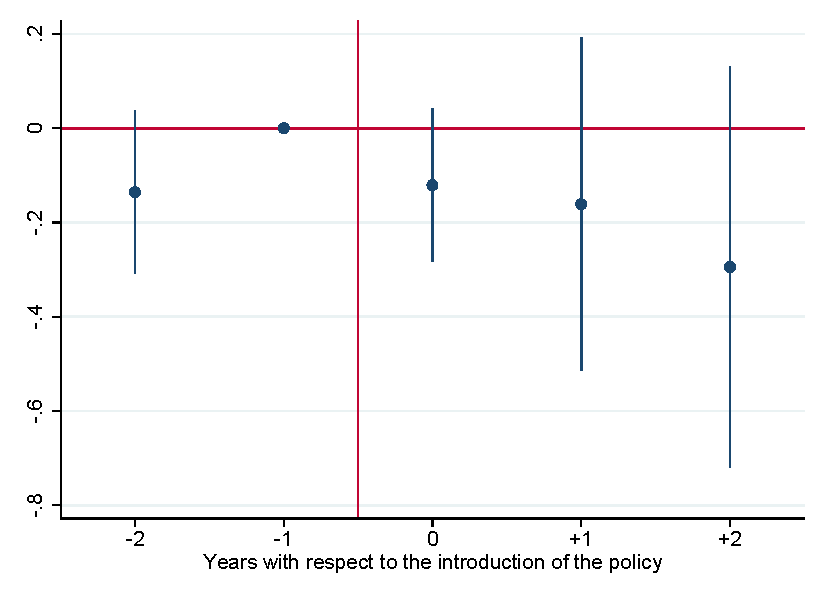
\includegraphics[width=47.2mm]{graphs/EventStudy-TaxCredit-Annual-Real.pdf}
   \label{fig:eventstudy-figure-annual-inputcredit}
}
\hspace{0mm}
\subfloat[Positive VAT Deposited]{   % ???
  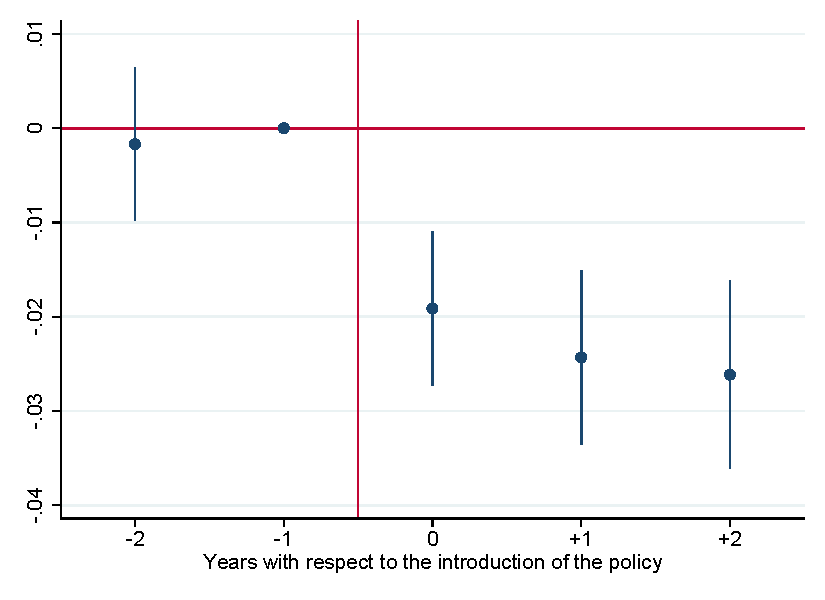
\includegraphics[width=47.2mm]{graphs/EventStudy-PositiveContribution-Annual.pdf}
   \label{fig:eventstudy-figure-annual-positivevat}
  }
\floatfoot{\footnotesize Notes: Graphical event-study analysis of the effect of third party verification policy on wholesalers compared to retailers. Confidence intervals were constructed with heteroskedasticity-robust standard errors, clustered at the firm level. The coefficient for the year ``-1'' (i.e., the year prior the policy) was normalized to zero. The regressions include firm fixed effects and time effects. The x axis indicates time, with annual observations and zero indicates the first year of the third party verification policy. Confidence intervals at the 95\% level. $N_W=32979$, $N_R=19515$. Coefficients in panel (a), (b), (c) and (d) are in million rupees with dependent variables price adjusted to the first year levels. \rupee 65 approximately equal to \$1. Pretrends are not statistically significant. }
\caption{Event Study: Wholesalers vs Retailers (Annual)}
\label{fig:eventstudy-figure-annual}
\end{figure}


\subsection{Quarterly Analysis}
\label[appendix]{subsec:eventstudy-quarter}

\begin{figure}[H]
\centering
\subfloat[VAT Deposited]{
  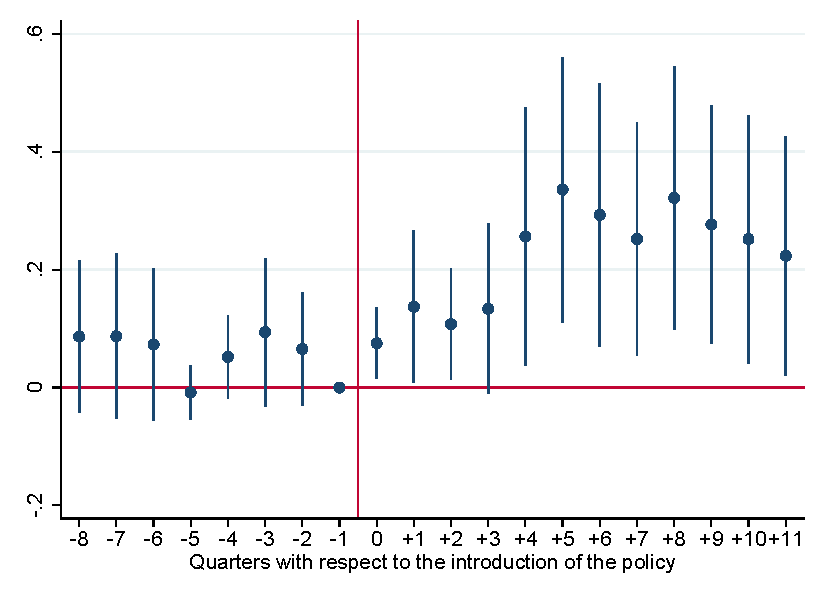
\includegraphics[width=47.2mm]{graphs/EventStudy-MoneyDeposited-Quarter-Real.pdf}
  \label{fig:eventstudy-figure-quarter-vatdeposited}
}
\subfloat[Output Tax - Input Credit]{
  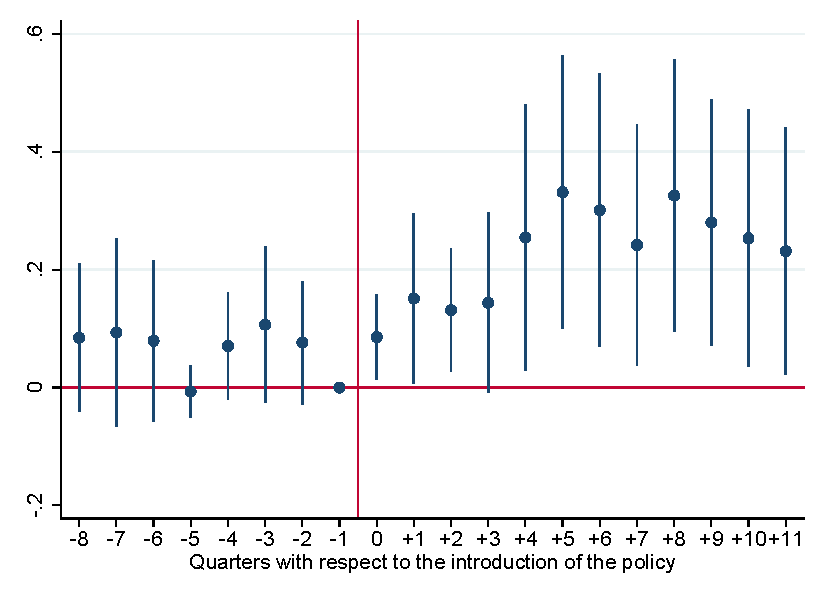
\includegraphics[width=47.2mm]{graphs/EventStudy-Diff-Quarter-Real.pdf}
   \label{fig:eventstudy-figure-quarter-diff}
}
\hspace{0mm}
\subfloat[Output Tax]{
  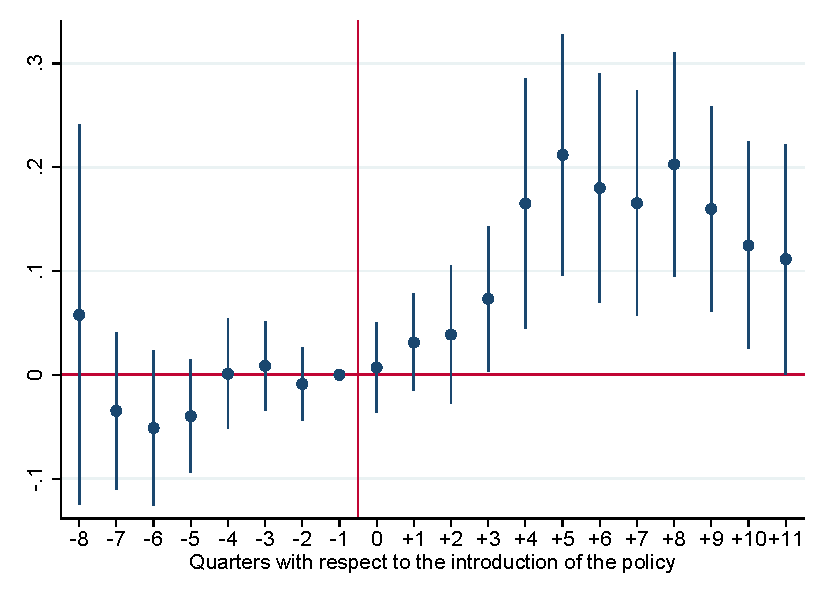
\includegraphics[width=47.2mm]{graphs/EventStudy-OutputTax-Quarter-Real.pdf}
   \label{fig:eventstudy-figure-quarter-outputtax}
}
\subfloat[Input Credit]{
  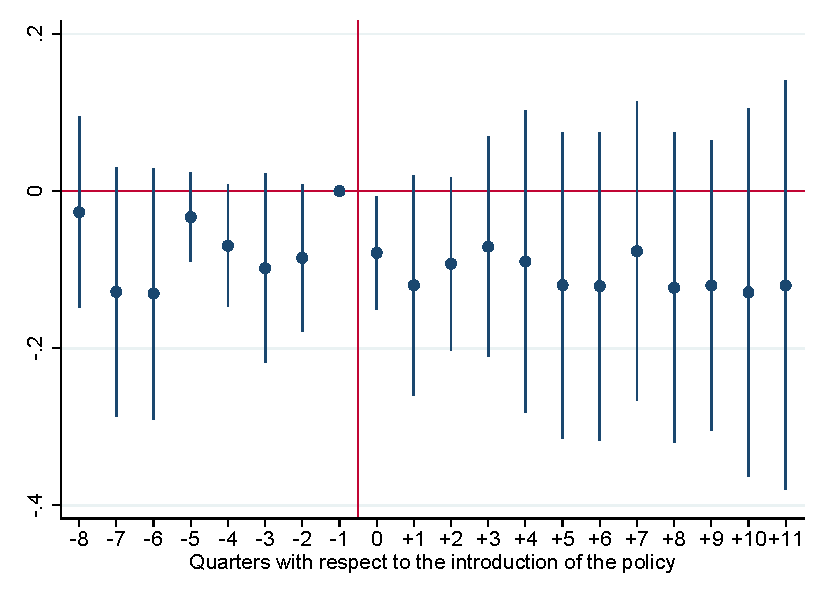
\includegraphics[width=47.2mm]{graphs/EventStudy-TaxCredit-Quarter-Real.pdf}
   \label{fig:eventstudy-figure-quarter-inputcredit}
}
\hspace{0mm}
\subfloat[Positive VAT Deposited]{   % ???
  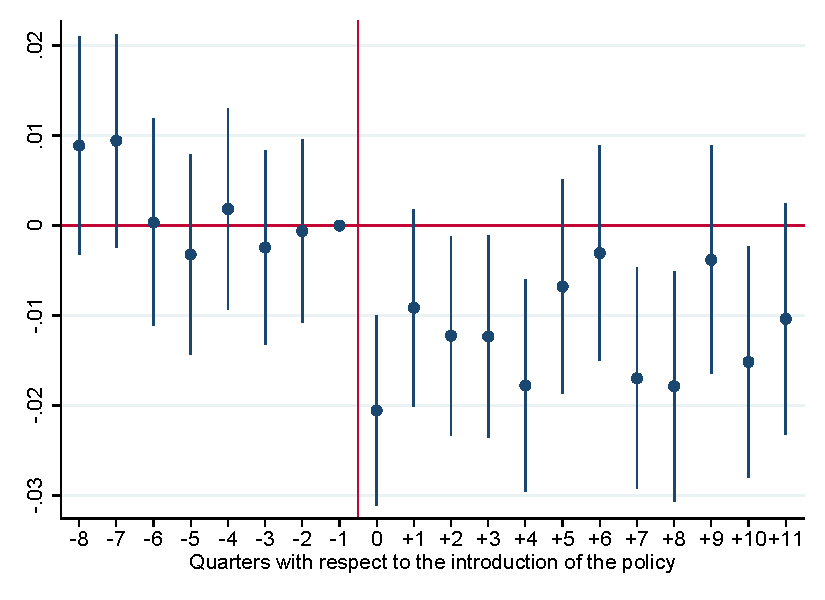
\includegraphics[width=47.2mm]{graphs/EventStudy-PositiveContribution-Quarter.pdf}
   \label{fig:eventstudy-figure-quarter-positivevat}
  }
\floatfoot{\footnotesize Notes: Graphical event-study analysis of the effect of third party verification policy on wholesalers compared to retailers. Confidence intervals were constructed with heteroskedasticity-robust standard errors, clustered at the firm level. The coefficient for the quarter ``-1'' (i.e., the quarter prior to the policy) was normalized to zero. The regressions include firm fixed effects and time effects. The x axis indicates time, with quarterly observations and zero indicates the first quarter of the third party verification policy. Confidence intervals at the 95\% level. $N_W=11482$, $N_R=15337$. Coefficients in panel (a), (b), (c) and (d) are in million rupees with dependent variables price adjusted to the first quarter of 2010 levels. \rupee 65 approximately equal to \$1. Pretrends are not statistically significant.}
\caption{Event Study: Wholesalers vs Retailers (Quarterly)}
\label{fig:eventstudy-figure-quarter}
\end{figure}

\pagebreak

\section{Other Results}

\begin{figure}[H]
\centering
\subfloat[Output Tax - Input Credit]{
  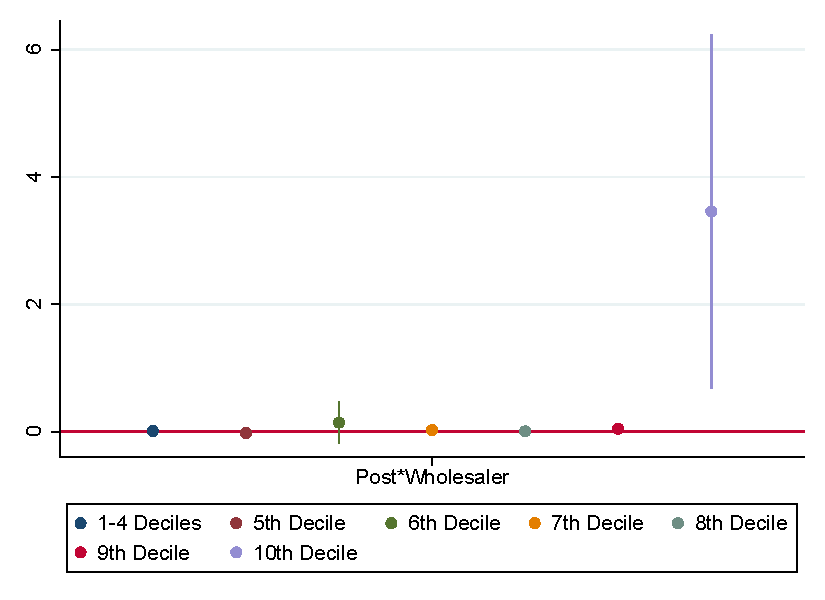
\includegraphics[width=50mm]{graphs/HeterogeneityDiff_Real.pdf}
}
\subfloat[Output Tax]{
  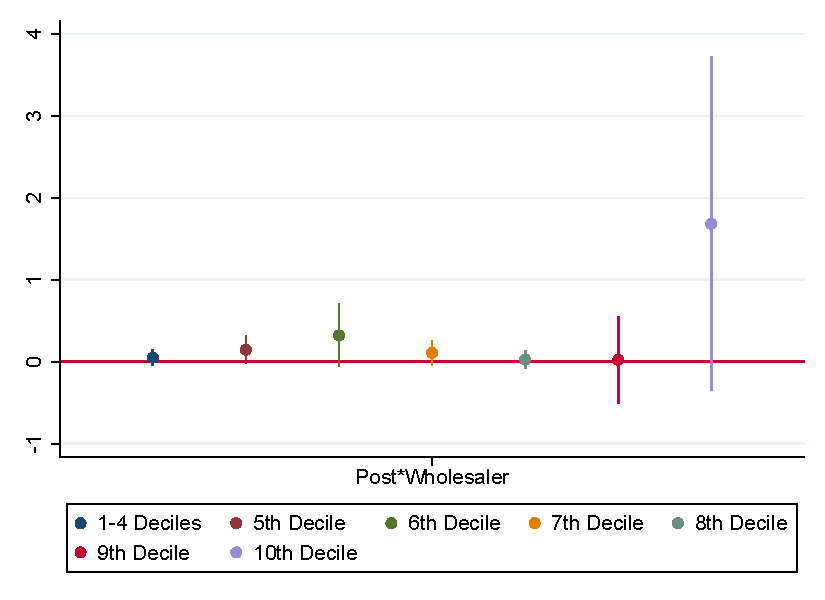
\includegraphics[width=55mm]{graphs/HeterogeneityOutputTax_Real.pdf}
}
\hspace{0mm}
\subfloat[Input Credit]{
  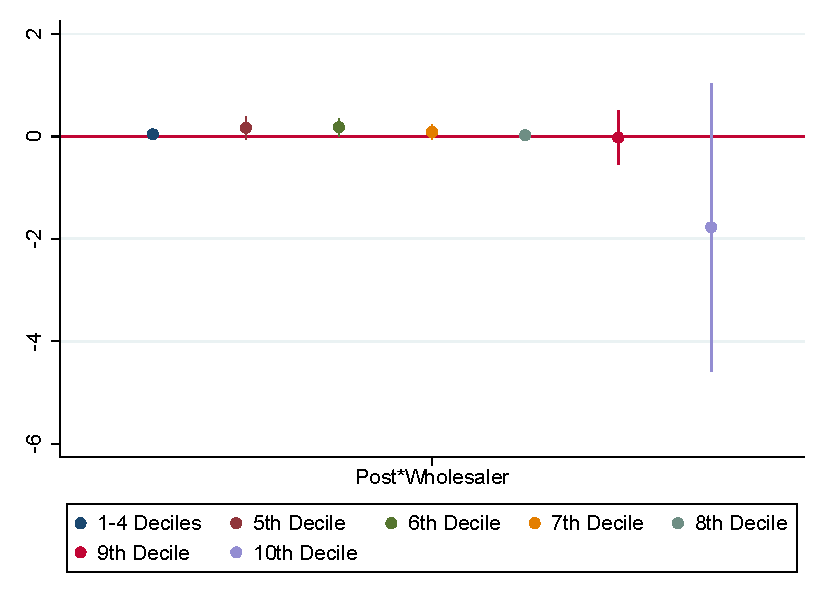
\includegraphics[width=55mm]{graphs/HeterogeneityTaxCredit_Real.pdf}
}
\subfloat[Positive VAT Deposited]{   
  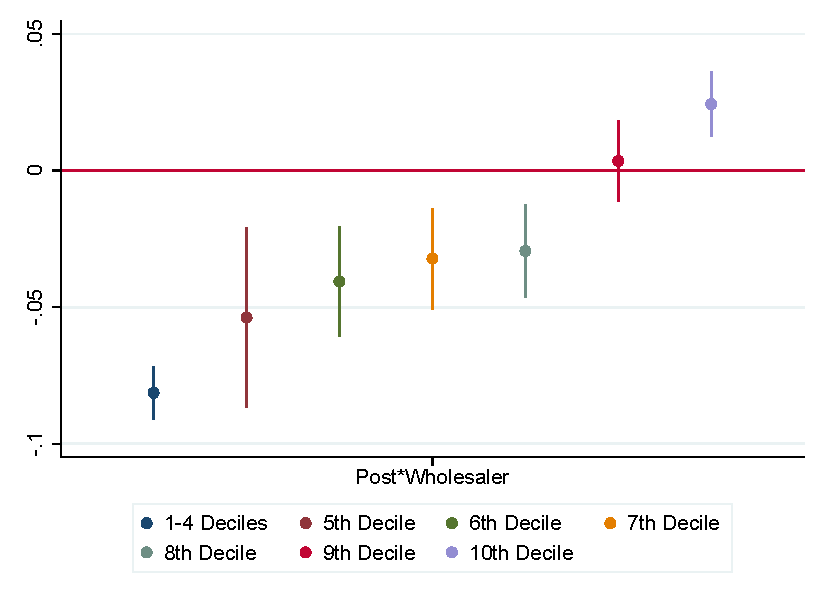
\includegraphics[width=55mm]{graphs/HeterogeneityPositiveContribution.pdf}
  }
\floatfoot{\footnotesize Notes: This figure plots the difference between wholesalers and retailers for different deciles, based on VAT remitted in the first year. The x axis indicates the decile. Confidence intervals at the 95\% level. Number of retailers is 32979 and number of wholesalers is 19515. Coefficients in panel (a), (b), and (c) are in million rupees, price adjusted to 2010-11 levels, with \rupee 65 approximately equal to \$1. Pretrends are not statistically significant.}
\caption{Heterogeneity Analysis: Wholesalers vs Retailers}
\label{heterogeneity-figure-annual}
\end{figure}
\pagebreak


\begin{figure}[ht]
\centering
\subfloat[Output Tax - Input Credit]{
  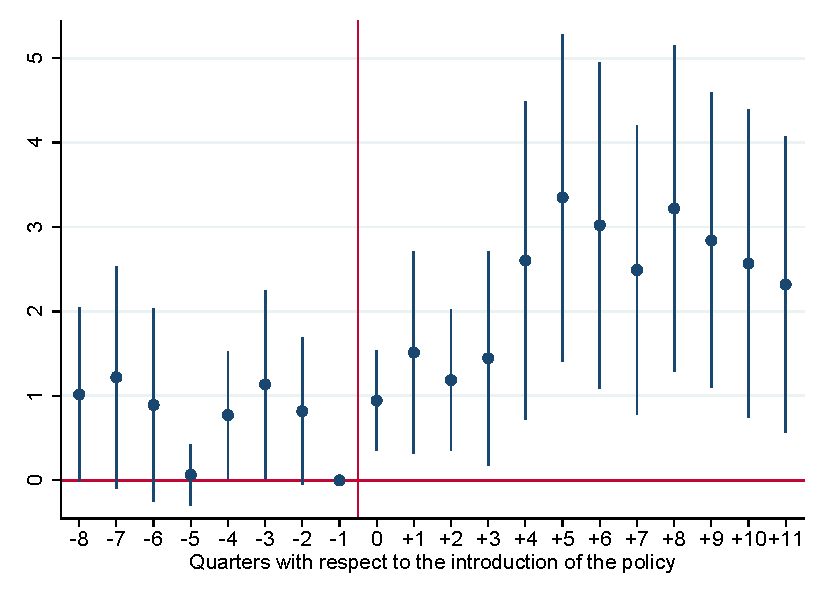
\includegraphics[width=55mm]{graphs/EventStudy-Diff-Quarter_TopDecile_Real.pdf}
  \label{fig:eventstudy-figure-quarter-diff-topdecile}
}
\subfloat[Output Tax]{
  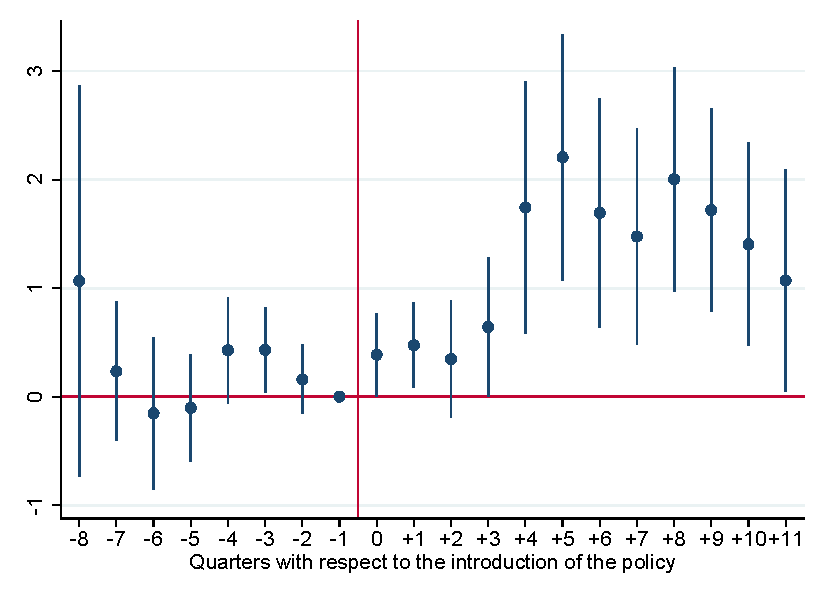
\includegraphics[width=55mm]{graphs/EventStudy-OutputTax-Quarter_TopDecile_Real.pdf}
  \label{fig:eventstudy-figure-quarter-outputtax-topdecile}
}
\hspace{0mm}
\subfloat[Input Credit]{
  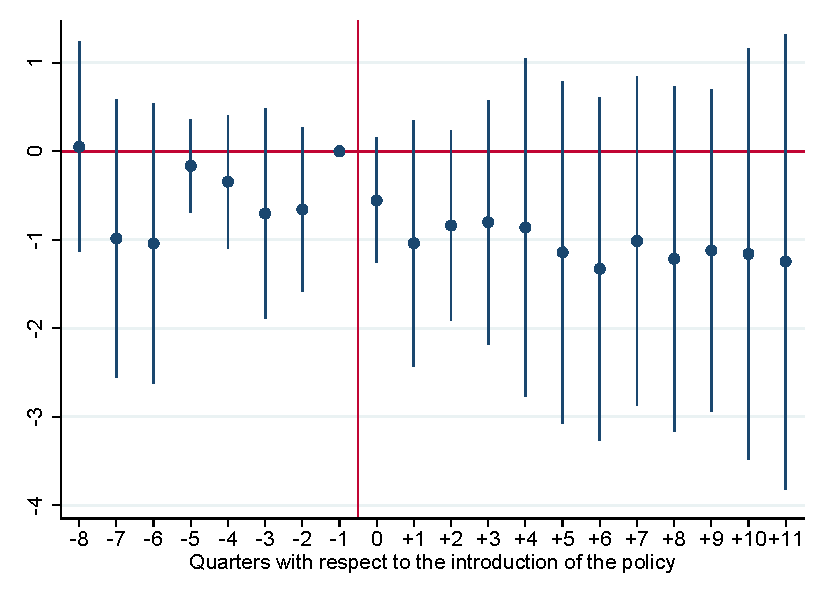
\includegraphics[width=55mm]{graphs/EventStudy-TaxCredit-Quarter_TopDecile_Real.pdf}
    \label{fig:eventstudy-figure-quarter-inputcredit-topdecile}
}
\subfloat[Positive VAT Deposited]{  
  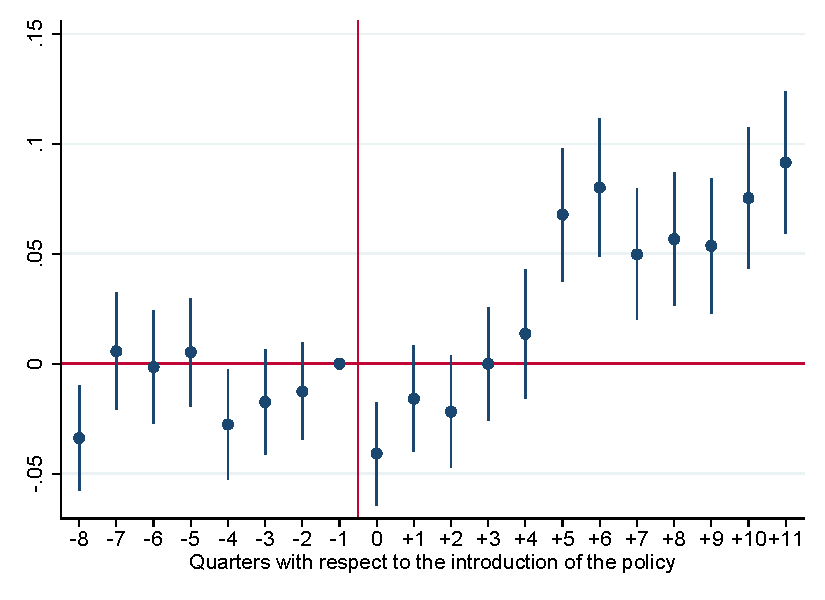
\includegraphics[width=55mm]{graphs/EventStudy-PositiveContribution-Quarter_TopDecile.pdf}
   \label{fig:eventstudy-figure-quarter-positivevat-topdecile}
  }
\floatfoot{\footnotesize Notes: Graphical event-study analysis of the effect of third party verification policy on wholesalers compared to retailers (for the top decile). Confidence intervals were constructed with heteroskedasticity-robust standard errors, clustered at the firm level. The coefficient for the group ``-1'' (i.e., the year prior the policy) was normalized to zero. The regressions include firm fixed effects and time effects. The x axis indicates time, with quarterly observations and zero indicates the first year of the third party verification policy. We have 20 quarters of data from 2010-11 to 2014-15. Confidence intervals at the 95\% level. Number of retailers is 1533 and number of wholesalers is 1148. Coefficients in panel (a), (b), (c) and (d) are in million rupees, price adjusted to Q1 of 2010-11 levels, with \rupee 65 approximately equal to \$1. Pretrends are not statistically significant.}
\caption{Quarterly Analysis for Top Decile: Wholesalers vs Retailers}
\label{fig:eventstudy-figure-quarter-topdecile}
\end{figure}



\section{Policy Execution: Other}
\label[appendix]{sec:execution}
%\setcounter{figure}{0}

\subsection{DiDiD: Proportion Registered Sales}
\label{subsec:ddd-rxprop}
\begin{figure}[H]
    \subfloat[VAT Deposited]{
      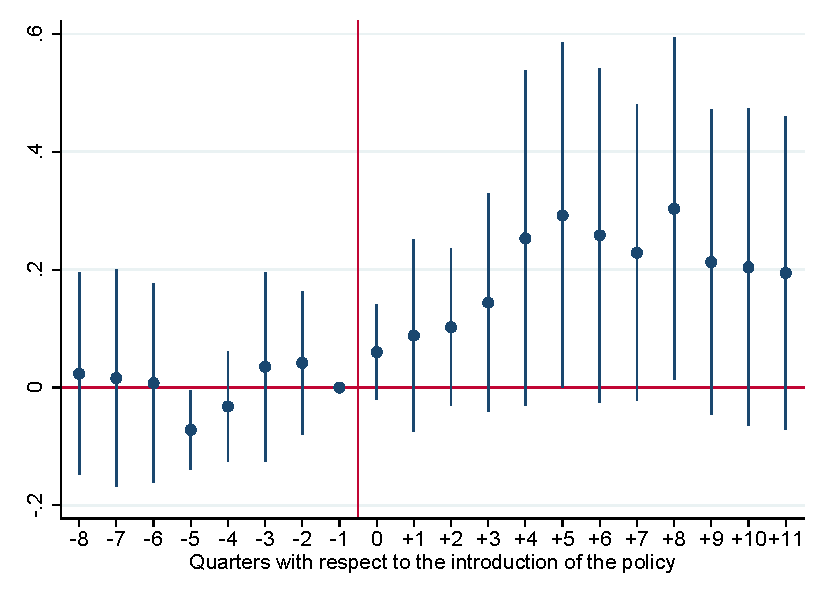
\includegraphics[width=47.2mm]{graphs/DDD_VATDeposited_Real.pdf}
    }
    \subfloat[Output Tax - Input Credit]{
      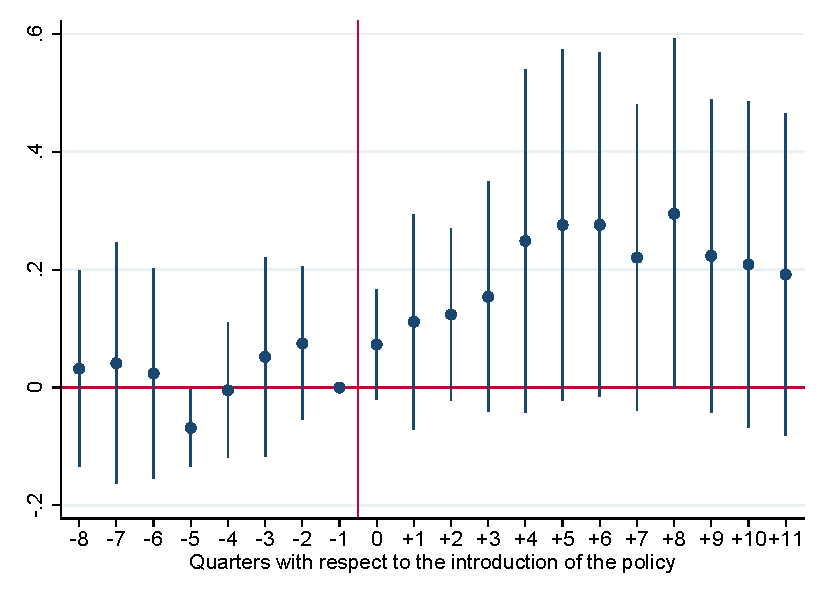
\includegraphics[width=47.2mm]{graphs/DDD_Diff_Real.pdf}
    }
    \hspace{0mm}
    \subfloat[Output Tax]{
      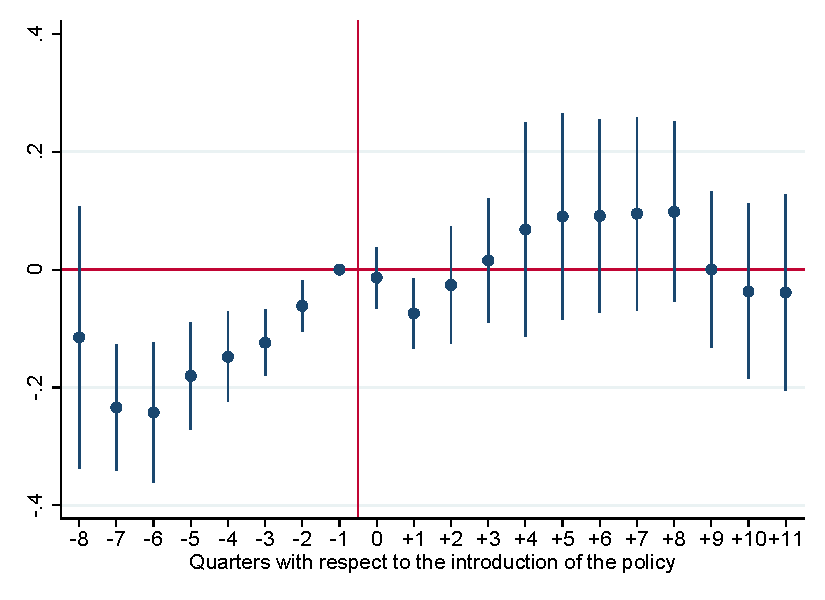
\includegraphics[width=47.2mm]{graphs/DDD_OutputTaxBeforeAdjustment_Real.pdf}
    }
    \subfloat[Input Credit]{
      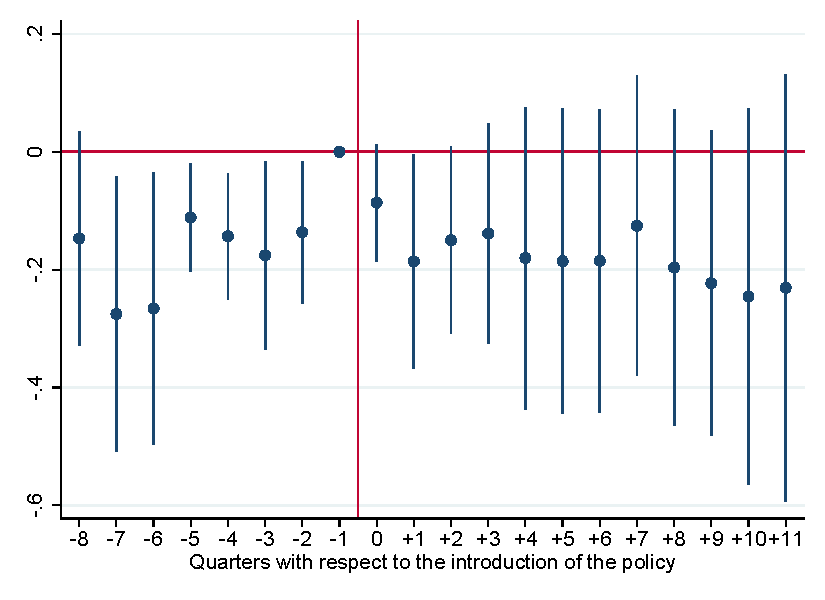
\includegraphics[width=47.2mm]{graphs/DDD_TaxCreditBeforeAdjustment_Real.pdf}
    }
    \hspace{0mm}
    \subfloat[Positive VAT Deposited]{   % ???
      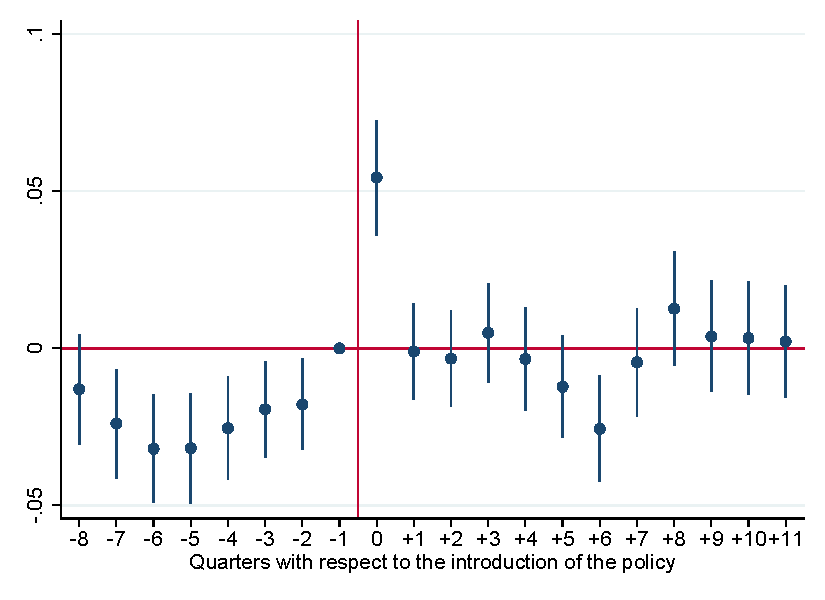
\includegraphics[width=47.2mm]{graphs/DDD_PositiveContribution.pdf}
      }
    \floatfoot{\footnotesize Notes: This figure plots the difference between wholesalers and retailers explained in \cref{eq:ddd}. The x axis indicates time, with quarterly observations and zero indicates the first quarter of the third party verification policy. Confidence intervals at the 95\% level. Number of retailers is 15337 and number of wholesalers is 11482. Coefficients in panel (a), (b), (c) and (d) are in million rupees, price adjusted to Q1 of 2010-11 levels. Pretrends are not statistically significant. }
    \caption{DiDiD: Wholesalers vs Retailers}
    \label[appendix]{ddd-figure-quarter}
\end{figure}

\pagebreak

\subsection{Revisions}
\label[appendix]{subsec:revisions}
%\todo[inline,caption={Aprajit: Revisions}, color=green]{The point of this section is to show that revision behavior post-policy is consistent with collusion on the part of retailers. At the moment we see (a) \# revisions go up immediately post-policy but then are down again by the end of the study and (b) the top percentile of wholesalers and retailers have about the same number of changes in revisions post policy as do the top 10\%.  The DID, however, shows that retailers revised their returns more than the wholesalers. Further, we see that these revisions were as likely to lead to decreases in tax liabilities as increases in tax liabilities for retailers (relative to wholesalers).}

\begin{figure}[ht!] 
\centering
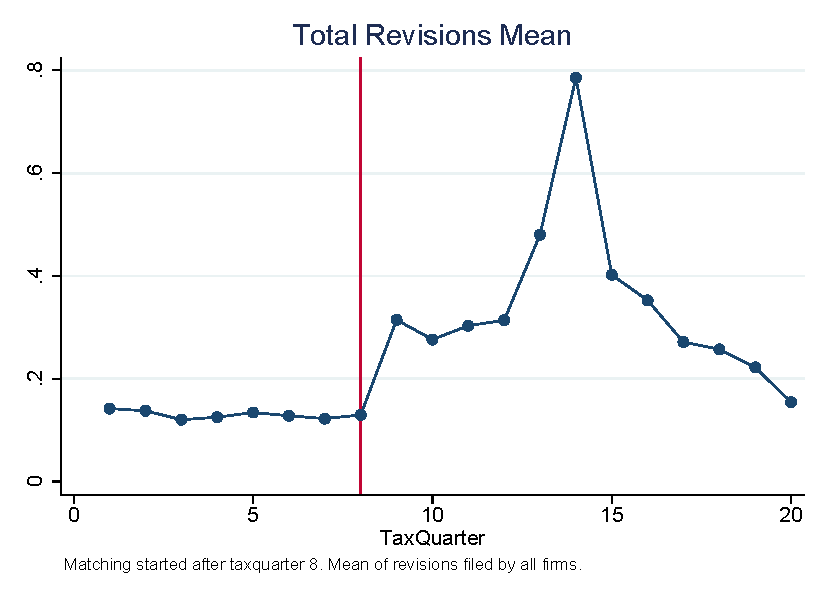
\includegraphics[width=0.75\textwidth]{graphs/RevisionTrends_All.pdf}
\caption{Mean Revisions of All Firms}
\label{fig:revision_all}
\end{figure}


Firms are allowed to revise filed returns until the end of next financial year. Before the start of the monitoring policy the average revision rates were around 13\% i.e. the mean of the total number of times a firm filed its returns was 1.13 (in Y1 and Y2). This revision rate was constant in the pre-period for both retailers and wholesalers. However, immediately after the introduction of the policy, the revision rates shot up to 30\% i.e. the mean of the total number of returns filed by a firm was now 1.3 (in Y3). As the issue mentioned between the consolidated and transaction returns was fixed in Y4, this number further shot up temporarily in Y4 (Q13) up to 78\% in Q14 and subsequently started coming down but remained higher than the average amount in Y1 and Y2.  This happened as now the firms had to file transaction level as well as the consolidated information (refer to \cref{fig:revision_all}). This behavior points towards two scenarios. Either the cost of complying with the tax policy is going up, or the firms are colluding and the increase in revisions is due to coordination costs. Either ways, it is important to think through the efficacy of the third party verification policy. Specifically, if most of the gain in revenue is from the top percentile of firms, then increasing the cost of compliance for firms across the board may not be cost efficient, both for the firms as well as the tax authority.

\begin{figure}[t!] 
%\centering
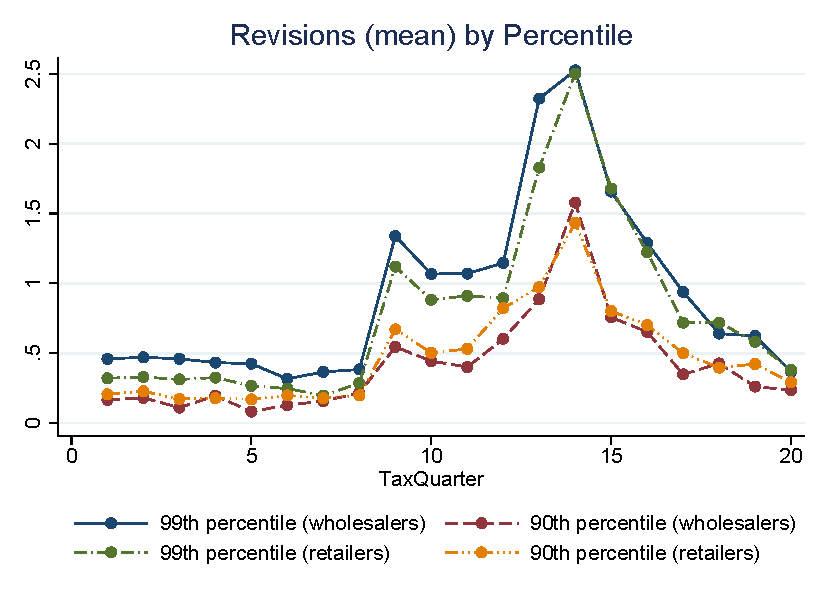
\includegraphics[width=0.75\textwidth]{graphs/RevisionsWholesSalerVsRetailerTopPercentile.pdf}
\caption{Mean Revisions of Wholesalers and Retailers}
\floatfoot{Describing revision trends by percentile. Comparing the firms in the top percentile with the firms in the 90th percentile}
\label{fig:revision_topdecile}
\end{figure}

There seems to be size based variation in the revision trends as well. When we compare wholesalers and retailers, we see that the 99th percentile (in terms of VAT deposited) of both the wholesalers and retailers revise their returns at a greater frequency than the 90th percentile firms (refer to \cref{fig:revision_topdecile}). This again hints towards the increase in revisions being driven by the increased cost of compliance.

\pagebreak
\subsection{Matching}
\label[appendix]{subsec:matching}

\begin{figure}[H] 
\centering
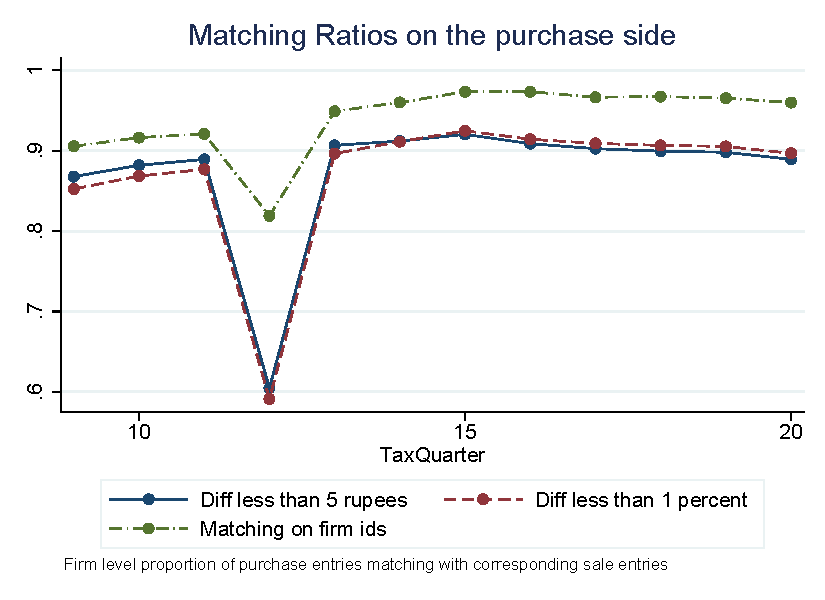
\includegraphics[width=0.75\textwidth]{graphs/AvgMatch_Purchases_alltypes.pdf}
\floatfoot{Firm level mean of purchases transactions matching with transactions declared by selling firms}
\caption{Matching on the Purchase Side for All Firms}
\label{fig:matching_purchases}
\end{figure}


In \cref{fig:matching_purchases}, \cref{fig:matching_sales}, \cref{fig:matching_retailerswholesalers}, and \cref{fig:matching_retailerswholesalers_sales}  we show the accuracy with which the sale and purchase transactions of firms match. Our ex-ante expectation was that after the policy was mandated, the transaction records will perfectly align. However, this does not seem to be the case. \Cref{fig:matching_purchases} shows  the average matches of the purchase declarations of a firm with the corresponding sale declarations of the selling firm. If we match only at the firm-id level, without considering the amount and tax rate declared, the most generous specification possible, the matching started around 90\% in the first year (Y3 of our dataset) and is around 96\% in year 5 of our analysis. 4\% of transactions are still unaccounted for ex-post. 


\begin{figure}[H] 
\centering
\caption{Matching on the Sales Side for All Firms}
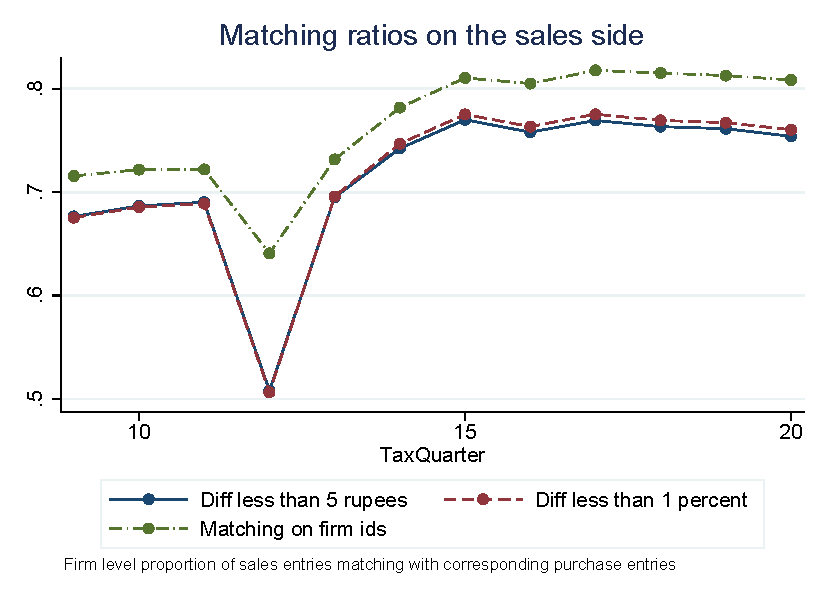
\includegraphics[width=0.75\textwidth]{graphs/AvgMatch_Sales_alltypes.pdf}
%\floatfoot{Firm level mean of sales transactions matching with transactions declared by buying firms}
\label{fig:matching_sales}
\end{figure}


We further narrow our analysis and consider the differences in amount. We try two specifications and the results are similar in both the specifications. We classify a transaction as a match if the difference in the total purchases declared by a firm (A) and the total sales declared by the corresponding firm (B) is less than 5 rupees or 1\% of the total purchases made by the firm A from firm B. One can assume that the mismatches that happen within this classification, are mostly driven by human error as the revenue implication is minimal. With this specification, the matching rate goes down to roughly 90\% across all the quarters. Therefore, roughly 10\% of the purchase declarations do not match in our sample in a serious manner. \Cref{fig:matching_sales} repeats the analysis but now we are comparing the sales transactions declared by  a firm with the corresponding purchase transactions of the buying firms. The results are similar except that now the firm-id level matching has gone down to 80\% across quarters. 



\begin{figure}[t!] 
\centering
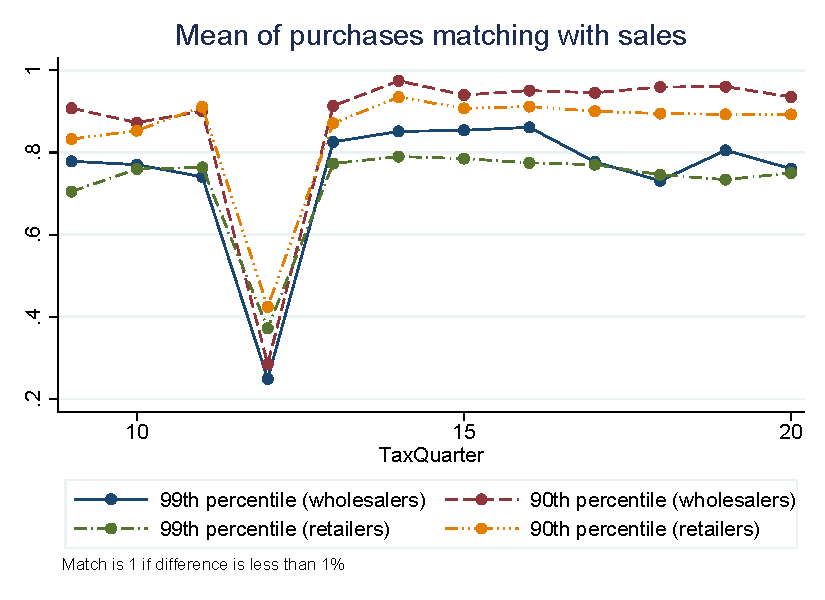
\includegraphics[width=0.75\textwidth]{graphs/AvgMatch_trend_DiffLessThan1percent.pdf}
\caption{Matching Analysis: Retailers Vs Wholesalers (Purchases, Top Percentile)}
\floatfoot{Describing revision trends by percentile. Comparing the firms in the top percentile with the firms in the 90th percentile}
\label{fig:matching_retailerswholesalers}
\end{figure}

In \cref{fig:matching_retailerswholesalers} and \cref{fig:matching_retailerswholesalers_sales} , we repeat the purchase and sale matching analysis but limiting ourselves only to our difference-in-difference sample of wholesalers and retailers. An interesting insight that is clearly visible is that matching for 90th percentile firms for both wholesalers as well as retailers is higher than the matching for the 99th percentile for the corresponding group. This is unexpected and further highlights that just the third party verification information may not be sufficient to reduce evasion and increase tax collections. Some sort of human monitoring effort on top of it is also needed, as despite this lower matching, most of the tax deposit growth is coming from the top percentile of wholesalers.

\begin{figure}[t!] 
\centering
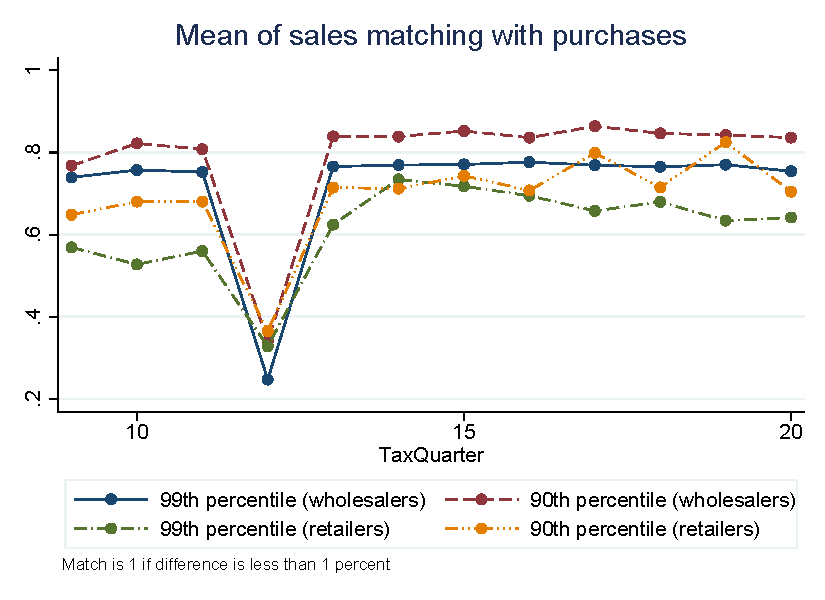
\includegraphics[width=0.75\textwidth]{graphs/SalesAvgMatch_trend_DiffLessThan1percent.pdf}
\caption{Matching Analysis: Retailers Vs Wholesalers (Sales, Top Percentile)}
\floatfoot{Describing revision trends by percentile. Comparing the firms in the top percentile with the firms in the 90th percentile}
\label{fig:matching_retailerswholesalers_sales}
\end{figure}

\pagebreak

\subsection{Consolidated vs Transaction Data}
\label[appendix]{subsec:consolidated_alignment}

\begin{figure}[H] 
\centering
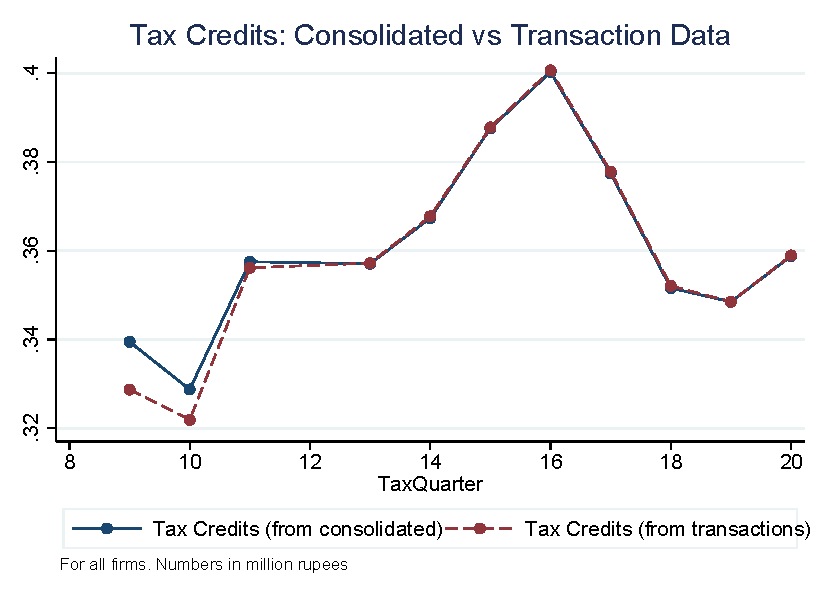
\includegraphics[width=0.75\textwidth]{graphs/TaxCreditComparison_allfirms_withoutq12.pdf}
\caption{Consolidated vs Transactional Data}
\floatfoot{In the first year, transaction data was not matched with the consolidated returns. Firms were clearly fudging, which was fixed in the subsequent years. We drop Q12 as unexplained behavior (possibly unrelated) is skewing the image.}
\label{fig:consolidated_transaction_minusq12}
\end{figure}

In the first year of the third party verification policy, transaction records filed were independently from the consolidated returns and these were not required to be consistent to each other. Therefore, it was possible that the aggregated transaction records did not match the consolidated returns -- which is what we observe. Specifically, total input credit claimed in the consolidated forms is on average higher than that implied by the annexures. The tax authority began requiring mechanical reconciliation of the two forms in the subsequent year at
which point such divergence ceases by definition -- see \cref{fig:consolidated_transaction_minusq12}).



%\end{appendices}
